\chapter{Analyse - État de l'art}
\label{ch:analysis}
Dans ce chapitre je vais m'intéresser aux différentes propositions d'implémentations de système de messagerie sécurisée afin de voir où en est l'état de l'art. Pour cela j'ai recherché les systèmes les plus connus tel que PGP et S/MIME mais aussi les implémentations de ces protocoles dans des clients mails tel que Protonmail ou Tutanota. J'élargis l'analyse à des protocoles plus orientés vers la messagerie instantanée comme Signal.
\section{Besoins d'un système de messagerie}
Cette section permettra de lister les besoins principaux d'un système de messagerie et l'utilisation qui en est faite habituellement.
\subsection{Besoins principaux}
Dans un système de mail les besoins principaux sont surtout de pouvoir consulter sa boite mail à tout moment avec les anciens et nouveaux mails reçus. De plus il est préférable de pouvoir envoyer des mails aussi. Ces envois peuvent avoir plusieurs propriétés et fonctionnalités. L'on pourrait envoyer un mail à de multiples destinataires et même sans que les uns et les autres sachent exactement à qui est envoyé le mail exactement (Copie cachées). Un client mail permet aussi d'envoyer des pièces jointes, celles-ci seront encodées au sein du message et envoyée avec. Un mail a aussi un état pour savoir s'il a déjà été lu ou non. Parmi l'utilisation simple d'un système de messagerie il y aussi le fait que l'on veut pouvoir voir ses mails de n'importe quel appareil à n'importe quel moment. 
\subsection{Détails techniques}
Afin d'établir le futurs notations utilisées ci-après et montrer le fonctionnement global d'un système de messagerie électronique je vais utiliser la figure \ref{fig:mailGlobal}. Dans cette figure l'on peut voir que 3 protocoles différents sont utilisés pour la gestion des emails ; SMTP, IMAP et POP3. Ces 3 protocoles sont utilisés par différents acteurs, le MUA (Mail User Agent), le MTA (Mail Transfer Agent) et le MDA (Mail Delivery Agent). Le MUA est en fait un client mail qui va s'occuper d'envoyer des mails ou de les recevoir (rechercher sur le MDA). Les MTAs sont les serveurs mails responsables du bon acheminement des mails. Ainsi les 3 protocoles énoncés plus hauts sont soit pour l'envoi et la transmission (SMTP) soit pour la récupération des messages (IMAP et POP3). Lors de l'envoi un MUA va simplement renseigner les destinataires du message ainsi que sa source, son sujet et son message puis le serveur va transmettre ces informations au MTA du domaine de destination qui s'occupera de le transmettre au MDA (souvent les 2 à la fois), celui-ci stocke les mails en attendant qu'un MUA fasses une demande via POP3 ou IMAP. IMAP est souvent préféré car les mails restent ainsi sur le serveur mail et est donc consultable depuis un autre appareil utilisant aussi IMAP. POP3 va plutôt télécharger les mails et les enlever du serveur et ils ne seront donc plus disponibles par le biais d'un autre appareil. Les MTAs sont des serveurs de transmission de données, transmises en clair jusqu'à l'introduction d'ESMTP et de la directive STARTTLS qui permet un niveau basique de sécurité entre 2 MTAS pour le transfert de mails. Cependant, si un MTAs est mal configuré et ne permet pas cette directive le mail transitera en clair. C'est dans ce contexte là et celui du stockage des mails en clair par le MDA que des solutions de chiffrement de mail en E2E (End to End - Chiffrement de bout-en-bout) ont vu le jour.
\begin{figure}[h!]
	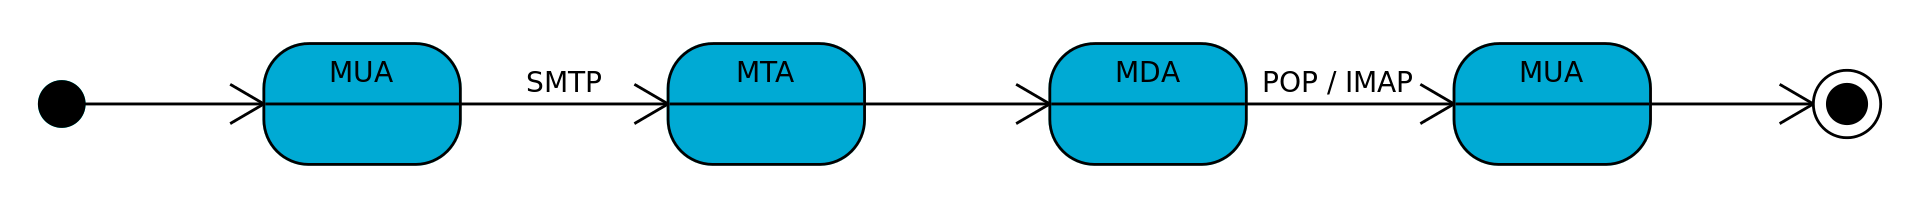
\includegraphics[width=14cm]{images/Etapes_envoi_email.png}
	\centering
	\caption{Le fonctionnement d'un système de mail~\cite{wiki:mailGlobal}}
	\label{fig:mailGlobal}
\end{figure}
\section{Protocoles existants}
Dans cette section je vais analyser les différents protocoles existants afin de sécuriser la messagerie électronique, ainsi que leur implémentation au sein de certains clients mails. De plus je m'intéresserait à la messagerie instantanée afin de voir s'il est possible d'implémenter cela dans un système de mails.
\subsection{PGP}
\paragraph*{Fonctionnement.}
PGP (Pretty Good Privacy ou Assez bon niveau de confidentialité) est un moyen de chiffrer des données (mails, fichiers, …). C’est une méthode de chiffrement hybride (utilise le chiffrement symétrique et asymétrique) qui fonctionne comme montré sur la Figure \ref{fig:PGP_101}. Comme on peut le voir, on tire une clé symétrique aléatoirement qui permettra de chiffrer notre mail avec un chiffrement symétrique comme AES. Ensuite, l'on va chiffrer cette clé symétrique à l'aide d'un chiffrement asymétrique, en utilisant la clé publique du destinataire.

\begin{figure}[h!]
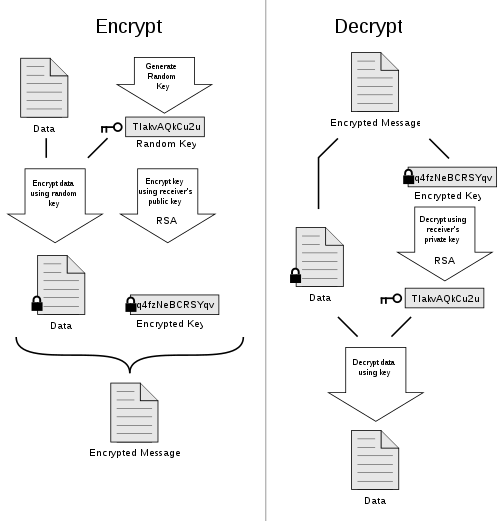
\includegraphics[width=10cm]{images/PGP_101.png}
\centering
\caption{Le fonctionnement global de PGP}
\label{fig:PGP_101}
\end{figure}

Ce fonctionnement hybride est expliqué par la lenteur d’un chiffrement asymétrique sur un certain nombre de données. Ainsi en chiffrant uniquement la clé symétrique qui a servi à chiffrer le message le déchiffrement est bien plus rapide et simple et est effectué typiquement avec un chiffrement symétrique tel qu’AES qui a le droit à des instructions dédiées dans certains processeurs. Contrairement à des chiffrements asymétriques qui sont plus contraignants. Mais il est nécessaire de passer par cette phase asymétrique, on a en effet besoin d'un secret partagé dès le début de la communication si cette méthode n'est pas utilisée.\\
Pour ce qui est des primitives cryptographiques proposées dans la RFC4880~\cite{RFC4880}, elle sont listées ci-après. Pour le chiffrement symétrique les primitives suivantes peuvent être utilisées : IDEA, TripleDES, CAST5, Blowfish, AES-128,AES-192, AES-256, Twofish-256. Pour les primitives asymétrique : RSA, ElGamal, DSA, ECDSA, Diffie-Hellman. La RFC spécifie aussi les formats de compression : ZIP, ZLIB, BZip2. Puis enfin, les algorithmes de hachage : MD5, SHA-1, RIPE-MD160, SHA256, SHA384, SHA512, SHA224 mais MD5 a été anoncé déprecié. Puis il faut savoir que pour chacune de ces catégories il y a 10 éléments réservés pour des primitives privées/expérimentales.\\
 Lorsqu'un mail est chiffré et signé avec PGP, il est d'abord hasher puis ce hash est signé avec la clé privée de l'utilisateur afin de faire une signature digitale, Le message et la signature sera alors chiffrée à l'aide la clé symétrique.\\
 
L'organisation d'un message PGP se fait via des "paquets" d'informations encodés en base64. La RFC définit bien ces types de paquets, leur fonctionnement et les différents codes associés. Sur le site \url{https://cirw.in/gpg-decoder/} l'on peut entrer un message et ainsi voir l'organisation d'un message, de clés publiques et de clés privées. Ainsi, je montre un exemple de mail envoyé à plusieurs destinataires dans la figure \ref{fig:PGP_DECODE}. Cela démontre comment fonctionnes PGP, en effet le message étant chiffré avec une clé symétrique le chiffré sera le même pour tout le monde. Mais afin que tout les destinataires puisses avoir la clé symétrique, la clé est chiffrée à l'aide des clés publiques des différents destinataires (et de la source, pour pouvoir la déchiffrer à l'avenir et ne pas conserver le mail en clair dans la boite d'envoi). À noter qu'avec l'option de \textit{blind copy} (option permettant d'envoyer à un utilisateur un mail sans qu'il sache qu'il a aussi été envoyé é un autre utilisateur), PGP \textit{leak} les receveurs des mails avec leur KeyID qui sera présent dans le message PGP\footnote{\url{https://crypto.stanford.edu/portia/papers/bb-bcc.pdf}}.\\
% TODO citer le papier ci-dessus au lieu du lien
\begin{figure}[h!]
	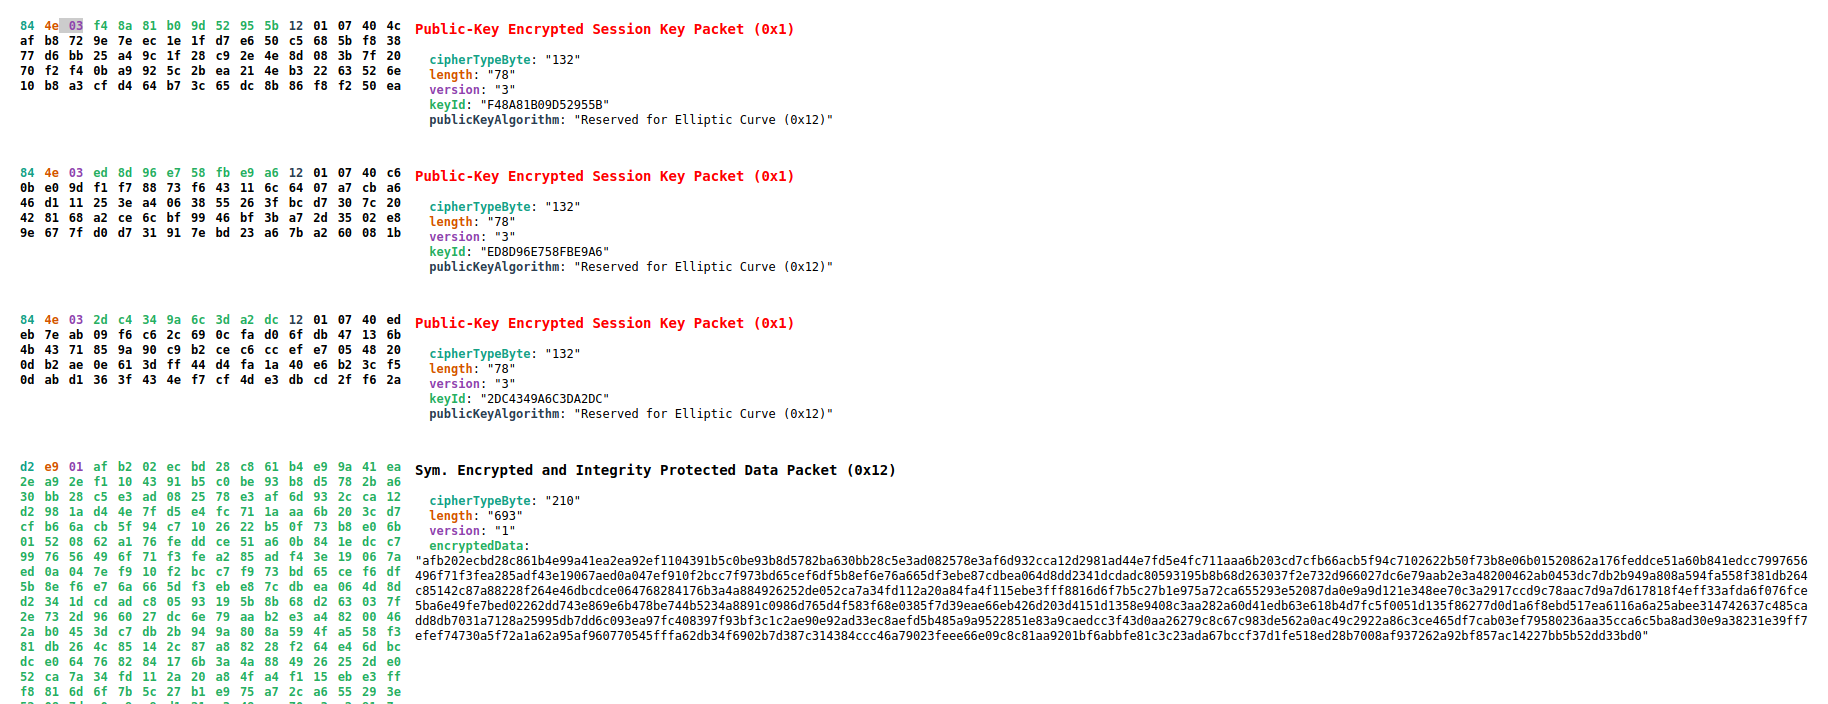
\includegraphics[width=14cm]{images/examplePGPDecode.png}
	\centering
	\caption{Exemple décodage d'un message PGP}
	\label{fig:PGP_DECODE}
\end{figure}
PGP utilise donc un système de clés publiques afin d'envoyer des clés symétriques. Comment obtient-on une clé publique pour envoyer notre message ?\\
Selon certaines utilisations les clés peuvent être obtenues via un serveur de clés, mais cela implique un parti tier auquel il faut faire confiance, ainsi ce qui peut être fait c'est aussi d'avoir son propre serveur de clés. Mais pour être sûr que tel clé appartienne bien à tel utilisateur, PGP a introduit dès ces débuts un système décentralisé de confiance appelé le "Web of Trust". Ainsi, un utilisateur pourra faire confiance à certaine clés d'autres utilisateurs et les signer, puis chacun des utilisateurs aura des clés de confiance et ainsi de suite. Cela permet d'avoir une toile de confiance entres les utilisateurs. Cependant, ce système est difficile à utiliser, il est nécessaire de faire attention à quelles clés les utilisateurs signent et approuvent. Surtout pour les nouveaux utilisateurs qui ne peuvent faire vérifier leurs clés publiques facilement et ne seront donc pas vérifier, c'est pour cela que des "fêtes" de signature de clés sont organisées afin de se rencontrer personnellement et vérifier que tel utilisateur est bien telle personne. Ces évènements sont d'ailleurs possible grâce aux Fingerprint des clés publiques, ce sont des chaines hexadécimales de 20 bytes permettant d'identifier une clé publique plus facilement.\\
SHA-1 est encore beaucoup utilisé pour les certificats d'identité et il a été prouvé que des attaques sur cet algorithme au niveau des collisions peuvent être faites~\cite{DBLP:journals/iacr/LeurentP20} donc à éviter d'utiliser également. Maintenant modifié dans les nouvelles version de GnuPG, ce n'est plus le standrad pour signer les clés publiques d'autres utilisateurs dans le Web Of Trust.\\
Dans la dernière spécification de PGP des moyens de créer des certificate authorities ont été ajouté afin d'avoir un système décentralisé de \textit{trust signatures} à différents niveaux et ainsi pouvoir se baser sur un système qui ressemble à un PKI mais avec une flexibilité sur les CAs (utilisateurs) auxquels on fait confiance ou non.
\paragraph*{Propriétés cryptographiques.}
PGP a surtout été crée pour fournir du \textbf{chiffrement de bout-en-bout} afin de résoudre les problèmes de transmissions en clairs entre les MTAs et le stockage des mails en clair dans les MDAs. Ainsi même lors d'une récupération de mails sur un serveur les mails seraient chiffrés. Ensuite PGP propose de signer ou non ses mails ce qui amène donc de la \textbf{répudiation} (si non-signé, le mail ne pourra pas être utilisé pour prouver qu'il a été envoyé par telle personne) et \textbf{non-répudiation} (mail signé, ainsi l'on peut prouvé que l'envoyeur a bien envoyé le mail).\\ 
Le problème qui est souvent reproché à PGP c'est qu'il n'implémentes pas de \textbf{Forward Secrecy}. La \textit{Forward Secrecy} permet d'affirmer que si l'on a une brèche à un instant $t$, et qu'un attaquant récupère notre clé privée, il ne pourra pas déchiffrer les anciens messages chiffrés avant l'instant $t$.
\paragraph*{Utilisation.}
Lors des tests l’utilisation la plus simple possible a été utilisée pour voir si un utilisateur lambda pouvait arriver à mettre en place ce genre de sécurité. Il s’est avéré que cela était assez simple au départ, mais dès lors que l'on veut envoyer un mail chiffré à un correspondant cela se complique. Uniquement l'installation d'un Add-On sur le logiciel de messagerie (Thunderbird dans ce cas) s’appelant Enigmail a été nécessaire. Ensuite Enigmail a généré les clés PGP (de manière totalement automatisée). Puis l'envoi d'un mail se fait simplement et rapidement via des icônes et des options dans le client mail. Cependant c’est très opaque et on ne sait pas ce qu'Enigmail fait réellement derrière les décors. L’utilisateur doit encore choisir s’il veut chiffrer ses mails ou non. De plus, Enigmail utilise Autocrypt, un système permettant d'envoyer la clé publique directement dans le mail. Pour les clés, Enigmail les envoie sur des serveurs de clés par défaut. Il va aussi interrogé ces serveurs si une clé publique pour un destinataire est disponible dessus lors du chiffrement d'un message. Ces serveurs sont les suivants : keys.opengpg.org (vks), hkps.pool.sks-keyservers.net (hkps), pgp.mit.edu (hkps). vks (Verifying Keyservers) et hkps (HTTP keyserver protocol over TLS) sont des interfaces avec des serveurs de clés afin d'enregistrer des nouvelles clés ou trouver une clé sur le serveur par différents moyens (email, key-id, fingerprint).
\subsection{S/MIME}
\label{protocols:SMIME}
\paragraph*{Fonctionnement.}
S/MIME se base sur un système de PKI (Public Key Infrastructure) pour chiffrer et signer des mails. 
\paragraph*{Propriétés cryptographiques.}
S/MIME est aussi crée pour établir un \textbf{chiffrement bout-en-bout} et ainsi éviter de révéler trop d'informations lors d'une brèche tel que dans un MDA. 
\textbf{Authentification} et \textbf{intégrité} du message en utilisant la signature digitale, en plus de \textbf{non-répudiation} grâce à celle-ci. Le fait d'avoir le message chiffré de bout en bout permet un certain respect de la vie privée, on ne peut voir les données envoyées.
\paragraph*{Utilisation.}
Pour utiliser S/MIME et avoir des exemples et références de certificats j'ai essayé 2 fournisseurs \textbf{gratuits} pour les certificats S/MIME.
J'ai testé  un plugin firefox qui permet d'avoir des certificats pour GMail et envoyer des mails signés et chiffrés à l'aide de S/MIME. La clé privée est générée par l'extension localement et n'est pas sauvegardée dans un cloud, il est possible de la sécurisé à l'aide dune passphrase. Cependant les certificats ne sont pas vérifier correctement comme on peut le voir à la réception dans MeSince (le prochain programme essayé) à la figure \ref{fig:SMIME_MeSinceProblem}. Le certificat utilise RSA avec SHA256 pour la signature des messages.
\begin{figure}[h!]
	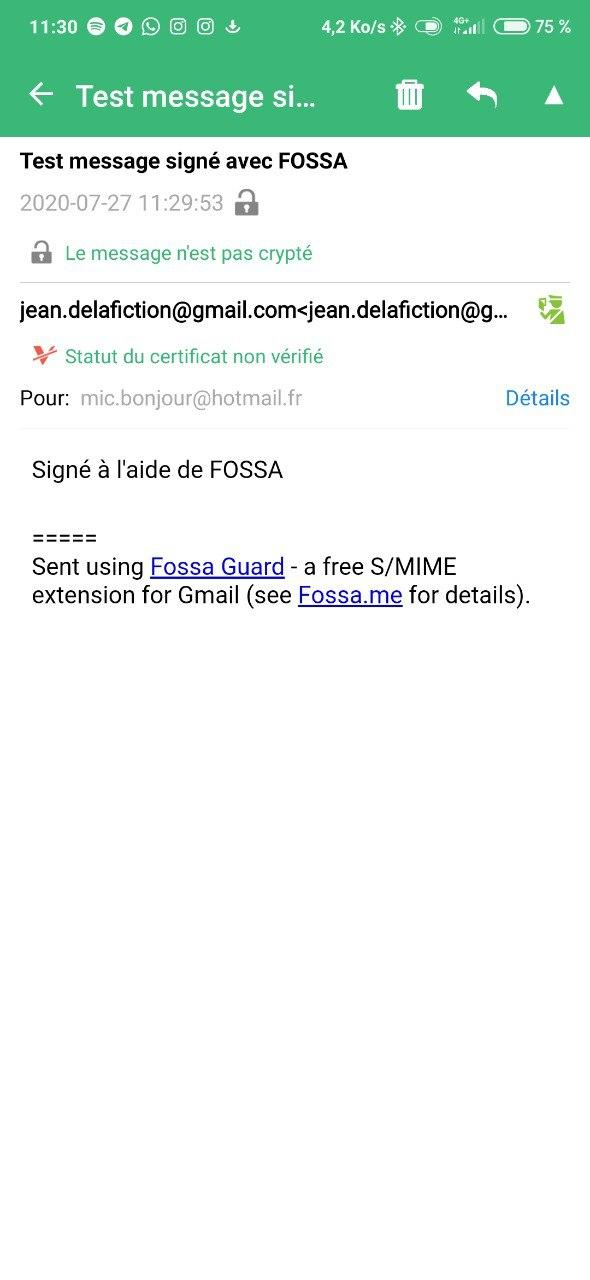
\includegraphics[width=10cm]{images/SMIME_FossaProblem.jpg}
	\centering
	\caption{Erreur de vérification pour Fossa}
	\label{fig:SMIME_FossaProblem}
\end{figure}
 Pour tester S/MIME, j'ai aussi lié un compte \url{https://www.mesince.com}. En effet, ce service permet d'utiliser S/MIME afin de chiffrer et signer ses mails, et ils fournissent les certificats, seulement il ne fonctionnait pas avec Gmail. De plus le service fourni n'a pas fonctionné pour se loguer et récupérer son certificat, ainsi le certificat a été généré et peut être utilisé par leur application mobile pour envoyer des mails signés et chiffrés mais je ne peux pas le voir. Sur l'application mobile il n'y a pas moyen de vérifier la clé générée.
Attention cependant le même problème qu'avec Fossa arrive comme je le montre dans la figure \ref{fig:SMIME_MeSinceProblem}, par contre l'avertissement n'est pas très voyant au sein de Gmail. Les certificats utilisent RSA avec SHA256 pour la signature des messages.
\begin{figure}[h!]
	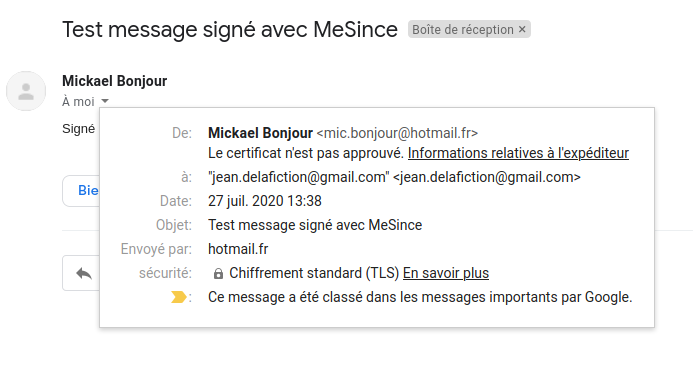
\includegraphics[width=15cm]{images/mesince_problem.png}
	\centering
	\caption{Erreur de vérification pour MeSince}
	\label{fig:SMIME_MeSinceProblem}
\end{figure}
 
 MeSince informe que la clé privée est automatiquement sauvegardée dans leur cloud sécurisé, ce qui n'est pas forcément une bonne nouvelle, de plus la clé est générée automatiquement donc aucune vérification de la part de l'utilisateur.
 Cependant ces 2 tests effectués ne représentent pas vraiment une utilisation réelle de S/MIME, en effet, le meilleur moyen de tester S/MIME aurait été d'avoir un nom de domain à soi et de générer des certificats S/MIME pour une adresse privée. Ensuite d'importer ses certificats et ses clés dans le client mail utilisés.
\subsection{PEP}
\paragraph*{Citation.}
\textit{By default, communications between pep peers always work end-to-end encrypted – no eavesdropping in between shall be possible by design.}
\paragraph*{Utilisation.}
pep assure un chiffrement de bout-en-bout par design, ils n'ont en effet pas de serveurs en soit et chiffre à l'aide d'un \textit{handshake} fait entres les deux personnes via des \textit{trustwords}. Ce sont des mots qu'il faut vérifier entres les deux partis afin d'être sûr que la connexion est bien authentifiée.
\begin{figure}[h!]
    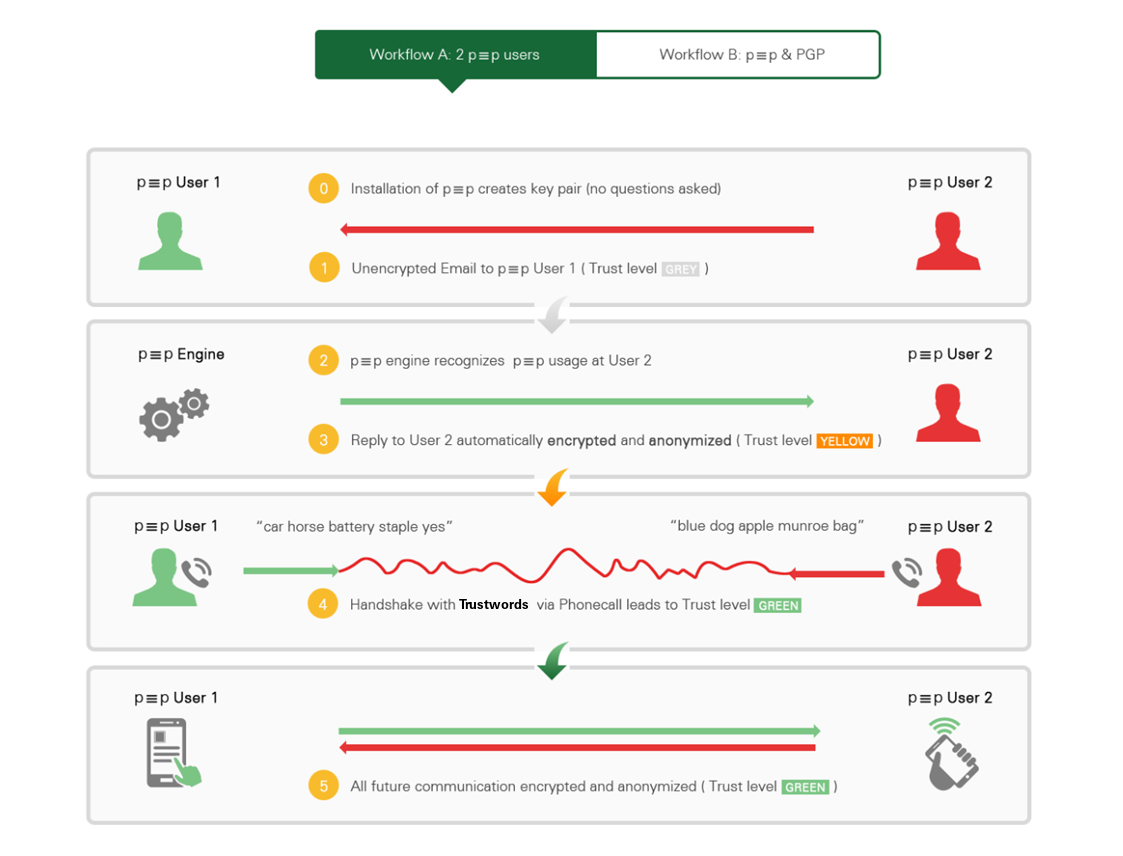
\includegraphics[width=15cm]{images/conceptualpEp.png}
    \centering
    \caption{Le fonctionnement global de pEp}
    \label{fig:PEP_global}
\end{figure}
-> à creuser mais à priori PEP utilise PGP pour le chiffrement des messages.

\section{Implémentations existantes}
Dans cette section je présentes certaines implémentations des protocoles discutés dans la section précédente, particulièrement PGP.
\subsection{Protonmail}
\paragraph*{Revendications.}
Protonmail revendique beaucoup de propriétés cryptographiques, tel que le zero-access encryption. Et l’end-to-end chiffrement + zero-knowledge pour les messages sécurisés, même avec leur fonctionnalité de (Chiffrement vers l'extérieur) utilisant AES256-GCM. 
Pour l'authentification Protonmail utilise une manière fortement sécurisée (SRP) pour ne pas avoir d'informations direct sur le mot de passe de l'utilisateur.
\paragraph*{Fonctionnement.}
Protonmail a plusieurs modes de fonctionnement dépendant du destinataire final. En effet de Protonmail à Protonmail les mails sont chiffrés à l'aide de PGP automatiquement. L'on peut utiliser Protonmail pour utiliser PGP si l'on a la clé de notre destinataire par exemple. Et l'on peut écrire un mail chiffré à quelqu'un qui n'utilise pas PGP grâce à une fonctionnalité de chiffrement vers l'extérieur.
Cette fonctionnalité enverra une URL au destinataire qui, en la consultant, pourra déchiffrer le mail en utilisant un mot de passe communiqué de manière sécurisées entres les deux partis auparavant.
\paragraph*{Open Source.}
Tout leur code est open-source afin d'avoir une validation externe, de plus ils ont un programme de Bug Bounty pour les chercheurs.
\subsection{Tutanota}
\paragraph*{Fonctionnement.}
Tout ce que j'ai vu pour le moment c'est que Tutanota utilise AES128-CBC ? Mais dans PGP ou ailleurs ?
%\subsection{Bitmessage}
\section{Attaque existantes}
Présentation des attaques faites sur les différents systèmes présentés jusqu'ici ainsi que leur fonctionnement global.
\subsection{Défauts webmails}
Selon un chercheur~\cite{DBLP:journals/iacr/Kobeissi18a} l'infrastructure de Protonmail aurait des failles via son webmail. Mais son papier est en fait plus général et parle des webmails en règle général.
Il part du principe que les serveurs de Protonmail ne sont pas des serveurs à faire confiance, pour ainsi prouver le zero-knowledge de Protonmail. Par contre, le fait qu'il ne peuvent pas être mis en confiance est un problème selon lui, car c'est ces serveurs qui vont délivrer le code d'OpenPGP afin de faire le chiffrement. 
Cela indique que si Protonmail était corrompu le fait d'avoir le code délivré par Protonmail pourrait avoir des effets néfastes. Comme p.ex l'extraction de la clé privée PGP. La conclusion est que dès le moment où vous avez utilisé une fois le webmail de protonmail la clé PGP est corrompue.
\subsection{EFAIL}
\label{attacks:EFAIL}
Malgré ces sécurités qui pourraient être mises en place à l’heure actuelle, une attaque nommée EFAIL~\cite{DBLP:conf/uss/PoddebniakD0ISF18} a été faite en 2018 et est toujours possible aujourd’hui(à vérifier / tester). En effet cette attaque a seulement été mitigée en évitant d’afficher les contenus HTML et les images dans boites mails de base. Car le problème vient de là principalement, des problèmes sont liés aussi aux modes de chiffrement utilisé (typiquement CBC et CFB) grâce à des "gadgets".
Cette attaque permet en fait d'injecter une image dans l'HTML du message (typiquement dans les headers du mail), puis faire en sorte de récupérer le contenu du message déchiffrer dans un paramètre de l'URL.
\section{Signal}
L'analyse s'est faite aussi pour la messagerie instantanée à cause de sa ressemblance avec la messagerie électronique. 
%Cela m'a finalement permis de me rendre compte que ce n'était pas des protocoles idéaux.
%TODO compléter l'analyse sur Signal
\subsection{Fonctionnement}
%TODO commenter la figure
\begin{figure}[h!]
	\centering
	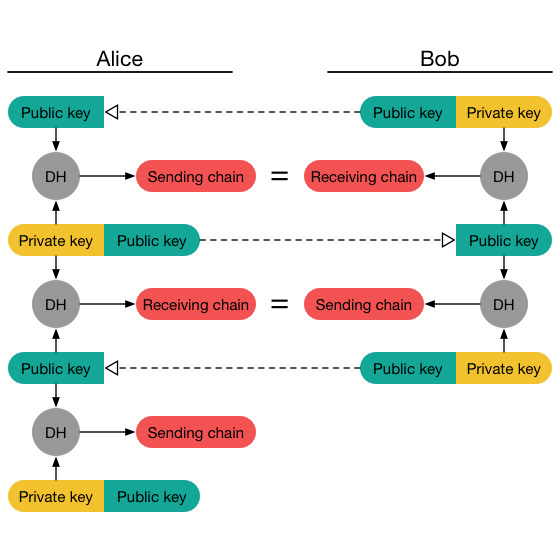
\includegraphics[width=8cm]{images/signalFonctionnement.png}
	\caption{Schéma fonctionnement de Signal\cite{doubleratchet}}
	\label{fig:signal}
\end{figure}
\subsection{Problèmes d'intégrations}
Le problème avec le protocole Signal quant à mes besoins niveaux mails est la \textit{forward secrecy} qui est très fort. En effet comme vu dans le chapitre précédent il utilise une clé par message grâce au \textit{Double Ratchet}. Cependant ce fonctionnement comporte un gros problème en rapport aux mails, en effet si l'on veut pouvoir récupérer les anciens mails reçus/envoyés cela devient vraiment compliqué. En effet, la \textit{forward secrecy} est une propriété utile dans un système de mail, mais faut pouvoir aussi récupérer les messages facilement si l'on connait la clé privée.
\section{Compromis}
Pour passer à l'implémentation concrète d'un nouveau protocole il faut faire des compromis et aller chercher dans des primitives moins connues.\\
Je suis tout de même rester sur un système de clés publiques comme PGP le fait. Cependant cette primitive a une identité propre à chaque clé publique ce qui évite un systéme de certificat trop complexe comme S/MIME.\\
De plus pour avoir une \textit{forward secrecy} l'on peut ajouter une notion de temps ou de token à l'ID pour chaque batch de messages.
\subsection{Résultats des recherches}
Comme mentionné avant les recherches ont beaucoup été orientées sur le protocole Signal qui a une très bonne forward secrecy, résilience et break-in recovery. Cependant le problème avec l'utilisation des mails c'est d'avoir envie de consulter tout ces mails depuis n'importe quel appareil. Ce n'est malheureusement pas le cas avec Signal à moins de conserver une \textit{root key} quelque part qui ferait s'effondrer les caractéristiques principales du protocole.\\
%TODO : Refaire ce paragraphe
S/MIME est la solution prédominante pour s'envoyer des mails chiffrés cependant il est compliqué de l'utiliser. Il et en effet difficile d'obtenir un certificat pour envoyer des mails et d'échanger avec une autre personne ayant S/MIME. De plus la complexité d'un systéme de PKI et l'overhead induit est assez conséquent.\\
En faisant quelques essais PGP de mon côté je me suis heurté à beaucoup de difficultés et de problèmes avec les clés PGP, notamment pour se les échanger mais pour envoyer ensuite ce n'est pas si complexe, le problème étant de bien voir les primitives utilisées pour chiffrer/signer notre email, en effet les solutions \textit{plug-and-play like} ne permettent pas une gestion précise des primitives cryptographiques utilisées, ce qui pourrait induire à des primitives par défaut non sécurisées, comme l'a démontré EFAIL(c.f. \ref{attacks:EFAIL}).
\section{Primitives}
Présentation des primitives considérées pour implémenter un système de messagerie sécurisée. Cette section présente un aperçu des primitives analysées, pourquoi je l'ai ou non retenue et leur fonctionnement en quelques mots.
\subsection{Primitives analysées}
Les primitives que j'ai analysé le plus sont présentées si après. Elles ont en commun de s'appuyer sur un principe basé sur l'identité. C'est très pratique dans un système de mail car une identité peut-être très vite définie par le biais d'une adresse email. Voici donc les technologies auxquelles je me suis intéressée et que je décris brièvement :
%TODO : Expliquer les différentes primitives
\begin{itemize}
	\item Certificateless PKC~\cite{DBLP:conf/asiacrypt/Al-RiyamiP03}
	\item HIBE - Hierarchical Identity Based encryption~\cite{DBLP:conf/eurocrypt/HorwitzL02}
	\item Identity based encryption~\cite{DBLP:conf/crypto/Shamir84}
\end{itemize}
%TODO à compléter
\subsection{Primitive choisie}
- Certificateless PKC~\cite{DBLP:conf/asiacrypt/Al-RiyamiP03}\\
 Cette primitive a été choisie car elle est similaire à de l'identity based encryption avec un ID pour désigner une clé publique. Le problème avec l'identity based encryption c'est le fait que le serveur central génère la clé publique et la clé secrète de l'utilisateur, cela amène ce qu'on appelle le \textit{key escrow} problème. C'est le fait qu'une entité connaisse à elle seule toutes les clés de tout les utilisateurs. Ce problème est résolu dans le certificateless en introduisant des \textit{Partial Private Keys} permettant d'avoir une clé secrète partiellement générée par le serveur (KGC - Key Generation Center) et par l'utilisateur puis assemblée pour former la clé privée seulement connue de l'utilisateur. De plus, cette primitive a l'avantage de ne pas introduire de certificats et ainsi évites la complexité d'une infrastructure de PKI (Public Key Infrastructure).
\section{Recherches sur la primitive}
\label{sec:primitiveSearch}
Dans cette section je vais introduire les détails techniques et les principes mathématiques utilisés. De plus, le choix de schéma parmi tous ceux analysés est détaillé ici. Ainsi que des précisions sur certains principes introduit par ce schéma.
% TODO : Présenter les différents types de pairings
\subsection{Principes mathématiques}
Les variantes de \textit{Certificateless Cryptography} choisies utilisent un concept appelé les \textit{pairings} ou \textit{bilinear map groups}.
Des groupes tels que $\mathbb{G}_1, \mathbb{G}_2, \mathbb{G}_T$ d'un ordre premier \textit{p} pour lesquels il existe un mapping $e : \mathbb{G}_1 \times \mathbb{G}_2 \rightarrow \mathbb{G}_T$ avec les propriétés suivantes :\\
1. Bilinéarité : $e(g^a, h^b) = e(g, h)^{ab}$ pour tout $(g,h) \in \mathbb{G}_1 \times \mathbb{G}_2$ et $a,b \in \mathbb{Z}$;\\
2. Pas de dégénérescence : $e(g,h) \neq 1_{\mathbb{G}_T} $ tant que $g,h \neq 1_{\mathbb{G}_{1,2}}$;
\subsection{À savoir}
\label{subsec:asavoir}
Avant d'analyser les différents schémas je vais présenter les différentes facteurs présentés dans les tableaux et ainsi établir une légende de ceux-ci expliquée.
\paragraph*{Types.}Les types présentés peuvent être soit \textbf{concret} soit \textbf{générique}. Les types concrets sont des schémas qui présentent leurs algorithmes en utilisant des calculs bien établis et présentent l'entierté du fonctionnement de leur schéma, tandis que les schémas présenté génériques peuvent s'appuyer sur d'autres problèmes et se baser sur des algorithmes déjà existants.\\
\paragraph*{Modèle de sécurité.} Ces modèles définissent sur quoi le schéma va se reposer pour établir sa sécurité et comment il va l'évaluer face à un adversaire. À nouveau il existe deux modèles présents dans les schémas analysés, le \textit{Random Oracle Model} et le \textit{Standard Model}. Le \textit{Random Oracle Model} se base sur des oracles aléatoires mais est un peu controversé, en effet l'aléatoire cryptographiquement sûr est difficile à atteindre, ainsi habituellement le \textit{Random Oracle Model} implémente ces oracles via des fonctions de hachage. Le modèle standard se base lui sur des problèmes mathématiquement difficiles tel que DDH (Decisional Diffie Hellman). \\
\paragraph*{Modèle d'adversaires.}
Pour évaluer les schémas de certificateless public key cryptography il y a différents niveaux de sécurité établis pour 2 types d'adversaires différents. Ces adversaires ont été décrits dans le papier d'Al-Riyami-Paterson~\cite{DBLP:conf/asiacrypt/Al-RiyamiP03} pour la première fois. Ces deux adversaires sont :\\
- Type I (\textit{outsider adversaries}) est appelé \textit{outsiders} et est permis de remplacer des clés publiques, obtenir des clés partiels privées, et des clés privées puis faire des requêtes de déchiffrements.\\
- Type II (\textit{honest but curious KGC}). L'adversaire de Type II est en fait un KGC connaissant la Master Secret Key et qui peut donc générer des PPK, obtenir des clés privées et faire des requêtes de déchiffrement tout en faisant confiance à ce KGC pour pas qu'il ne remplace de clés publiques.\\
Pour chacun des types d'adversaires il existe différents niveaux de sécurité :\\
%TODO : Remplir avec infos du livre sur les différents niveaux
\subsection{Schémas Certificateless de Chiffrement}
Pour choisir parmi les nombreux schémas existants en certificateless pour le chiffrement j'ai établi un tableau comparatif des différentes manières de faire, inspiré de~\cite{bookIntroCertificateless}. En suivant ce tableau je me suis rendu compte que la construction de Dent-Libert-Paterson~\cite{DBLP:conf/pkc/DentLP08} était probablement la plus adaptée en vue des propriétés qu'elle présentait. Le tableau se trouve en annexe \ref{ch:fichiers}.

\subsection{Détails techniques}
Les détails techniques sur le chiffrement avec la \textit{Certificateless Cryptography}.
Le chiffrement se base sur le problème difficile \textit{The Decision 3-Party Diffie-Hellman Problem} (3-DDH). \\C'est de décider si $T =g^{abc} ayant (g^a, g^b, g^c, T) \in \mathbb{G}_4$.\\
Pour expliquer les détails techniques je vais ici montrer les calculs faits dans le schéma choisi~\cite{DBLP:conf/pkc/DentLP08} et les expliquer, cependant dans le schéma il est noté les calculs avec $\mathbb{G} \times \mathbb{G} \rightarrow \mathbb{G}_T$ mais il est mentionné que c'est facilement adaptable pour $\mathbb{G}_1 \times \mathbb{G}_2 \rightarrow \mathbb{G}_T$ ce que j'ai fait. De plus, la conversion vers un groupe additif (travaillant sur les courbes elliptiques) est faite afin que les calculs ici puissent être lus avec mon implémentation :\\
\textbf{Setup($1^k, n$) :} Avec $\mathbb{G}_1, \mathbb{G}_2, \mathbb{G}_T$ avec un ordre $p > 2^k$. $g$ est un générateur de $\mathbb{G}_1$. Ensuite  $g_1 = g * \gamma$ pour un $\gamma \leftarrow  \mathbb{Z}_p^*$ aléatoire. Puis $g_2 \leftarrow \mathbb{G}_2$. Deux vecteurs (U,V) seront tirés aléatoirement dans $\mathbb{G}_2^{n+1}$ en tant que fonctions de hash notés :
\[F_u(ID) = u' \sum_{i=1}^{n} u_j^{i_j}\quad\mathrm{and}\quad F_v(w) = v' \sum_{i=1}^{n} v_j^{w_j}\]
L'on va aussi prendre une fonction de hash résistante aux collisions : $H : \{0,1\}^* \rightarrow \{0,1\}^n$. Au final notre $mpk$ (master public key) est :
\[mpk \leftarrow (g, g_1, g_2, U, V)\]
Et le $msk$ (master seret key) est $msk \leftarrow g_2*\gamma$.\\
\textbf{Extract($mpk, \gamma, ID$) :} On prend $r \leftarrow \mathbb{Z}_p^*$ puis on retourne $d_{ID} \leftarrow (d_1, d_2) = (g_2*\gamma + F_u(ID)*r, g*r)$\\
\textbf{SetSec($mpk$) :} Retourne un secret aléatoirement choisi $x_{ID} \leftarrow \mathbb{Z}_p^*$.\\
\textbf{SetPub($x_{ID}, mpk$) :} Retourne $pk_{ID} \leftarrow (X,Y) = (g*x_{ID}, g_1*x_{ID})$.\\
\textbf{SetPriv($x_{ID}, d_{ID}, mpk$) :} On choisit $r' \leftarrow \mathbb{Z}_p^*$ puis on reprends $(d_1, d_2) \leftarrow d_{ID}$ et l'on va prendre en secret key : 
%TODO : Revoir si assez complet :
\[sk_{ID} \leftarrow (s_1, s_2) = (d_1*x_{ID} + F_u(ID)*r', d_2*x_{ID} + g*r')\]
Avec $sk_{ID}$ étant la clé secrète de l'utilisateur, donnée par l'Extract (notre Partial Private Key) et la valeur secrète de SetSec.\\
\textbf{Encrypt($m, pk_{ID}, ID, mpk$) :} Pour chiffrer $m \in \mathbb{G}_T$, l'on va reprendre $(X,Y) \leftarrow pk_{ID}$. Pour chiffrer ce message on va tiré aléatoirement $s \leftarrow \mathbb{Z}_p^*$ pui calculer : 
\[C = (C_0, C_1, C_2, C_3) \leftarrow (m + e(Y, g_2)*s, g*s,F_u(ID)*s, F_v(w)*s )\]
Où $w \leftarrow H(C_0,C_1, C_2, ID, pk_{ID})$.\\
\textbf{Decrypt($C, sk_{ID}, mpk$) :} L'on peut reprendre $(C_0,C_1,C_2,C_3) \leftarrow C$ et la clé privée $(s_1, s_2) \leftarrow sk_{ID}$. Afin d'accélérer le déchiffrement le calcul suivant peut être fait en tirant une valeur aléatoire $\alpha \leftarrow \mathbb{Z}_p^*$ :
\[m = C_0 + \frac{e(s_2 + \alpha*g, C_2 )*e(\alpha*g, C_3)}{e(C_1, s_1 + F_u(ID)*\alpha + F_v(w)*\alpha)}\]
Qui donnera $m$ le texte en clair si le chiffré était bien formaté ou un élément aléatoire dans $G_T$.
\subsection{Schémas Certificateless de Signature}
%TODO : Expliquer Malicious KGC (Type II -> à renseigner (voir dans le livre)) et mettre tableaux
Pour choisir parmi les nombreux schémas certificateless pour la signature j'ai établi un tableau comparatif des différentes manières de faire inspiré de~\cite{bookIntroCertificateless}. En analysant les différentes possibilités dans ce tableau il y a peu de solutions se dégage, en effet l'on peut voir que beaucoup de schémas de signature sont cassés, mon choix s'est porté au final sur la construction de Zhang et Zhang~\cite{DBLP:conf/acns/ZhangWXF06} pour des signatures robustes en Certificateless. J'ai pris cette construction car elle est résistante au Malicious KGC (si le KGC a été setup avec des paramètres vulnérables) datant de 2006 et n'a pas été cassée depuis. Le tableau se trouve en annexe \ref{ch:fichiers}.
\subsection{Détails techniques}
Les détails techniques sur la signature avec la \textit{Certificateless Cryptography}.
La signature se base sur le problème difficile \textit{The Computational Diffie-Hellman Problem} (CDH). \\Ayant $P, aP, bP$ où $a,b$ aléatoires $\in \mathbb{Z}_q^*$ il n'est pas possible de trouver $abP$.\\
Pour expliquer les détails techniques je vais ici montrer les calculs faits dans le schéma choisi~\cite{DBLP:conf/acns/ZhangWXF06} et les expliquer. Cependant dans le papier original le groupe bilinéaire de couplage choisi est de forme $\mathbb{G}_1 \times \mathbb{G}_2 \rightarrow \mathbb{G}_T$ avec un \textit{pairing} $e(g,h)$ avec $g \in \mathbb{G}_1, h \in \mathbb{G}_2$ alors que le papier annonce une construction tel que $\mathbb{G} \times \mathbb{G} \rightarrow \mathbb{G}_T$.\\
\textbf{Setup($1^k $) :} Tout d'abord l'on va prendre les groupes d'ordre $q$ énoncés auparavant. Puis on choisit un générateur $P \in \mathbb{G}_1$. La \textit{master secret key} va être choisie aléatoirement $s \in \mathbb{Z}_q^*$. Puis la clé publique calculée : $P_{pub} = sP$. Finalement, trois fonctions de hash distinctes $H_1, H_2, H_3$ vont être choisies, chacune d'elle \textit{mappant} de $\{0,1\}^*$ à $\mathbb{G}_2$. Pour cela j'ai choisi de faire du \textit{Hash Domain Separation} comme expliqué dans le Chapitre \ref{ch:impl}. L'on définit les $\mathbf{params} = (\mathbb{G}_1,\mathbb{G}_2,\mathbb{G}_T,e,q,P,P_{pub},H_1,H_2,H_3)$\\
\textbf{Partial-Private-Key-Extract($params, s, ID_A$) :} Pour avoir la \textit{Partial Private Key} ($D_A$) de l'user $A$ avec l'identité $ID_A$. Calculer $Q_A = H_1(ID_A)$. Alors $D_A = sQ_A$.\\
%TODO : Compléter
\textbf{Set-Secret-Value :} La valeur secrète $x \in \mathbb{Z}_q^*$ est tirée aléatoirement.\\
\textbf{Set-Public-Key($params, x$) :}  La clé publique $PK_A$ de l'utilisateur $A$ est $PK_A = xP$.\\
\textbf{Set-Private-Key($params, D_A, x$) :} La clé privé $SK_A$ de l'utilisateur $A$ est calculée comme ceci $SK_A = (D_A, x)$.\\
\textbf{CL-Sign($params, m, ID_A, SK_A$) :} Tout d'abord $r \in \mathbb{Z}_q^*$ est tiré aléatoirement puis on calcules les 2 composantes de la signature :
\[ U = rP\]
\[V = D_A + rH_2(m, ID_A, PK_A,U) + xH_3(m, ID_A, PK_A)\]
Ainsi ces composantes forment la signature $\sigma = (U,V )$.\\
\textbf{CL-Verify($params, PK_A,  m, ID_A, \sigma$) :} Tout d'abord l'on va calculer $Q_A = H_1(ID_A)$ puis effectuer ce calcul afin de vérifier la signature :
\[e(V,P) == e(P_{pub}, Q_A)*e(U, H_2(m, ID_A, PK_A,U))*e(PK_A, H_3(m, ID_A, PK_A)) \]
\section{État de l'art}
Dans cette section je vais analyser et comparer les différentes solutions trouvées utilisant la \textit{Certificateless Cryptography} dans une implémentation concrète pour sécuriser des envois d'emails. J'ai trié les articles suivants par date de publication afin de voir comment les suivants ont repris les technologies etc.
\subsection{Email Encryption System Using Certificateless Public Key Encryption Scheme}
Analyse de l'article~\cite{DBLP:conf/itcs2/ErYTG12}.
\paragraph*{Description.} Cet article présente une façon de faire pour chiffrer les mails à l'aide de \textit{Certificateless Cryptography}. Il va d'abord comparer 6 schémas pour choisir celui à utiliser par rapport à ses propriétés. Ensuite il va comparer les différents algorithmes au niveau du temps avec une implémentation simple en J2SE. 
\paragraph*{Détails techniques.} Les détails techniques ne sont pas très fourni dans cet article, en effet, il est mentionné uniquement le choix du schéma (Whang-Huang-Yang). Puis une comparaison des temps entre les différent algorithmes de la primitive. Finalement ils présentent la différence de temps entre le chiffrement du message via le certificateless et via une clé AES qui est chiffrée avec le certificateless.
\paragraph*{Conclusion.} Ce papier nous conforte dans l'idée de l'utilisation d'AES pour la rapidité du chiffrement qui va avec cette primitive. Cependant, ils n'expliquent pas comment la clé AES est prise et chiffrée réellement. Une implémentation existe en J2SE mais je ne l'ai pas trouvée. Le schéma choisi l'a été pour son avantage de ne pas utiliser les \textit{pairings} et est donc plus rapide. Puis parmi les autres schémas qui n'utilisent pas les \textit{pairings} à ce moment là, un est de type générique (c.f. sous-section \ref{subsec:asavoir}) et l'autre est vulnérable aux \textit{outsider attacks} (c.f. sous-section \ref{subsec:asavoir}).
\subsection{An End-To-End Secure Mail System Based on Certificateless Cryptography in the Standard Model}
Analyse de l'article\footnote{\url{https://www.ijcsi.org/papers/IJCSI-10-2-3-264-271.pdf}}~.
\paragraph*{Description.} Cet article présente une façon de chiffrer et signer dans un système de mail avec le schéma original de \textit{Certificateless Cryptography} à savoir le schéma d'Al-Riyami et Paterson~\cite{DBLP:conf/asiacrypt/Al-RiyamiP03}. Un article complet définissant bien le contexte de mails et formalisant pour la première fois un moyen de chiffrer et signer des mails avec de la \textit{Certificateless Cryptography}. Cela en expliquant dans les détails comment ils feraient, sans implémentations citées de ce schéma.
%TODO A voir, j'ai l'impression qu'il y a une erreur dans le papier pour le déchiffrement de t*
\paragraph*{Détails techniques.} Les détails techniques intéressant dans ce papier est la manière d'encapsuler la clé de chiffrement du message. Sinon le reste s'appuie sur le schéma d'Al-Riyami et Paterson.
Pour établir une clé de chiffrement symétrique afin de chiffrer le mail l'n va tout d'abord tirer une valeur aléatoire $t \in \mathbb{Z}_p$ puis la chiffrer avec CL-PKC en utilisant la clé publique du destinataire $t* = Enc_{P_B}$. Ce $t^*$ sera envoyé avec l' email. Pour en tirer une clé symétrique on va établir : $K_{AB} = tx_AP_B$ à l'aide de la clé privée de la source et la clé publique du destinataire et enfin la valeur aléatoire tirée auparavant. Puis l'on va calculer la clé symétrique $K = H_2(Q_A||Q_B||K_{AB})$.
\paragraph*{Conclusion.} Ce papier est assez complet concernant la partie fonctionnement des mails en globalité et offres une bonne idée pour la construction d'une clé symétrique par mail envoyé. Cependant la mise en place de la clé symétrique et la preuve de son fonctionnement n'est pas très explicitée. D'ailleurs il y a selon moi une erreur dans le papier original pour la logique de déchiffrement de $t^*$ et de la récupération de la clé symétrique. De plus, le système de signature d'Al-Riyami et Paterson a été cassé par~\cite{DBLP:conf/cans/HuangSMZ05}.
\subsection{Practical Implementation of a Secure Email System Using Certificateless Cryptography and Domain Name System}
Analyse de l'article~\cite{DBLP:journals/ijnsec/BalakrishnanR16}.
\paragraph*{Description.} Ce papier traite le problème de la même façon que le précédent mais essaies d'aller plus loin dans les détails d'un implémentation à plus grande échelle (utilisation DNS). Il reprend le même schéma et les mêmes principes pour la création de la clé symétrique de chiffrement. Le même schéma de signature est présent aussi, qui est cassé rappelons-le. Le but serait d'avoir une entrée DNS similaire au DKIM déjà utilisé pour les emails afin d'informer les utilisateurs quelle adresse donne es clés publiques du domaine en question.
\paragraph*{Détails techniques.} Beaucoup de détails concernant les domain policies qui pourraient être appliqués aux domaines pour la distribution des clés publiques. Proposition d'utiliser les headers d'emails pour transmettre la signature de l'email et informer le destinataire si l'email est chiffré ou non et de transmettre les IDS utilisés et le TImestamp utilisé. En effet, l'introduction d'un timestamp est proposé ici pour avoir un temps d'expiration au mail. Les Domain Policies sont là pour informer les utilisateurs si les emails de ce domaines doivent être signés/chiffrés ou non.
\paragraph*{Conclusion.} Une implémentation est citée utilisant la librairie MIRACL et en utilisant le C++ comme langage de programmation. L'implémentation est citée comme extension \textit{Thunderbird} en C++ / Javascript. Mais il n'y a pas de réel guide pour implémenter cela au monde réel avec des exemples de configuration DNS et autres. Pas vraiment d'explications sur l'utilisation d'une multitude de KGC ou un seul central, comment les synchroniser et autres... Par contre beaucoup d'explications sur comment pourrait fonctionner une entrée DNS afin d'informer aux utilisateurs où aller pour récupérer les clés publiques des utilisateurs du domaine en question et des policies qui pourraient s'appliquer à ce domaine.
%TODO à compléter, signifier intéressant
\subsection{PriviPK : Certificate-less and secure email communication}
Analyse de l'article~\cite{DBLP:journals/compsec/AlSabahTLSD17}.
\paragraph*{Description.} Cet article propose une implémentation très concrète utilisant CL-PKC pour communiquer de manière sécurisée dans la messagerie électronique. Il attaque beaucoup d'aspects que les autres papiers n'ont pas mentionnés comme la \textit{key transparency}. Le papier insiste sur la transparence du protocole pour l'utilisateur afin qu'il n'ait pas d'opérations fastidieuses à faire (comme c'est le cas dans PGP et S/MIME par exemple). Ce papier s'appuie sur un système de \textit{key agreement} proposé dans la littérature de la cryptographie basée sur l'identité.
\paragraph*{Détails techniques.} CONIKS serveur, authentification via les clients mails déjà existants (gmail et yahoo), mise en place d'un système de key agreement id-based repensée pour le certificateless.
\paragraph*{Conclusion.} Ce papier est assez intéressant et c'est la seule véritable implémentation que j'ai trouvée, il y a un repo sur github. Cependant il s'appuie sur du \textit{key agreement}. Comme le prochain système d'ailleurs. Par ailleurs, il insiste sur la transparence et sur l'utilisation des authentifications déjà présentes sur les clients emails.
\subsection{A certificateless one-way group key agreement protocol for end-to-end email encryption}
Analyse de l'article~\cite{DBLP:conf/prdc/YehSDSSW18}.
\paragraph*{Description.} Dans cet article les auteurs présentent un moyen d'avoir une clé partagée entre n-partis et avec un seul message, ce qui permet dans un système de mail d'avoir qu'à envoyer un mail avec les informations nécessaires pour recomposer la clé partagée. Cette clé partagée est utilisée afin de chiffrer le mail et de l'envoyer ensuite avec les informations nécessaires à la création de la clé partagée. De plus, le système est n-parti, cela veut dire que l'on peut envoyer le mail à n personnes et le chiffrer avec la même clé. On enverra juste pas les mêmes informations de créations de la clé partagée à tous.
\paragraph*{Détails techniques.} Pour ce qui est des détails techniques on peut voir que le principe est de créer une clé partagée à l'aide des différents ID et clés publiques des destinataires. On aura une sous-clé $x_i$ pour chaque utilisateur $i$. L'on va construire un $y_i = x_0 \dots x_{i-1} + x_{i+1} \dots x_n$ pour un utilisateur où l'on additionnera tout les $x$ des utilisateurs sauf de l'utilisateur $i$. Ainsi à la réception du message l'utilisateur pourra recréer la clé partagée en faisant $y_i + x_i = x_0 + \dots + x_n = K$. Ce $K$ sera ensuite utilisé pour chiffrer le mail.
\paragraph*{Conclusion.} Ce système est simple et efficace mais ne permets pas la signature des éléments nécessaires à la création de la clé partagée, l'on peut donc envisager des DOS afin qu'un utilisateur ne puisses plus lire ces messages. Cependant c'est une construction intéressante se basant sur un \textit{key-agreement} via le \textit{Certificateless Cryptography} et non pas sur ses possibilités de chiffrement/signature.



